% Figure 1: system overview (TikZ, compiles with the paper; no external assets).
\begin{figure}[t]
\centering
\resizebox{\textwidth}{!}{%
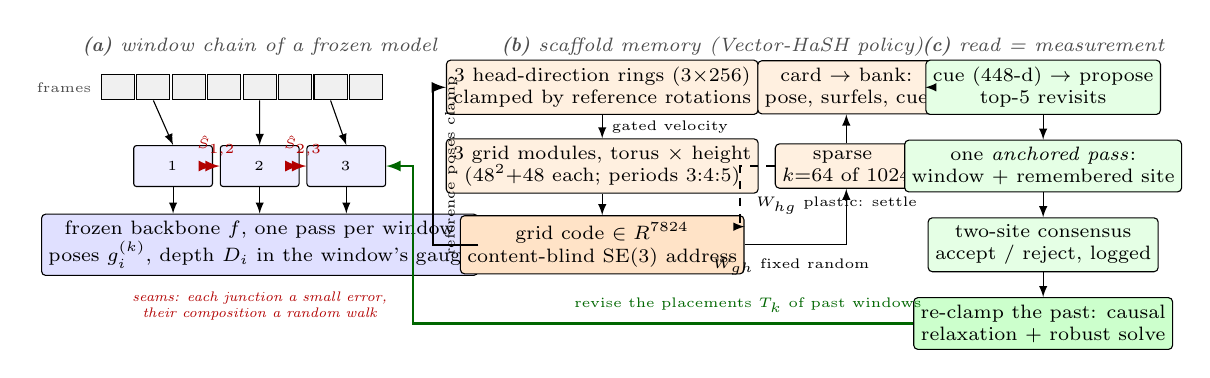
\begin{tikzpicture}[
  font=\scriptsize, >=latex,
  box/.style={draw, rounded corners=1.5pt, align=center, inner sep=2.5pt, minimum height=5.2mm},
  frame/.style={draw, fill=gray!12, minimum width=4.2mm, minimum height=3.2mm, inner sep=0pt},
  win/.style={draw, rounded corners=1pt, fill=blue!7, minimum width=10mm, minimum height=5.2mm, align=center, inner sep=1.5pt},
  mem/.style={draw, rounded corners=1.5pt, fill=orange!12, align=center, inner sep=2.5pt, minimum height=5.6mm},
  read/.style={draw, rounded corners=1.5pt, fill=green!10, align=center, inner sep=2.5pt, minimum height=5.6mm},
  lbl/.style={font=\scriptsize\itshape, text=black!70}]
% ---------------- (a) frozen backbone on windows, glued by Sim(3) ----------------
\foreach \i in {0,...,7} { \node[frame] (f\i) at (0.45*\i, 0.15) {}; }
\node[lbl, anchor=east, font=\tiny] at (f0.west) {frames};
\node[win] (w1) at (0.7, -0.85) {$\cW_1$};
\node[win] (w2) at (1.8, -0.85) {$\cW_2$};
\node[win] (w3) at (2.9, -0.85) {$\cW_3$};
\draw[->] (f1.south) -- (w1.north); \draw[->] (f4.south) -- (w2.north); \draw[->] (f6.south) -- (w3.north);
\node[box, fill=blue!12, minimum width=34mm] (bb) at (1.8, -1.85) {frozen backbone $f$, one pass per window\\ poses $g_i^{(k)}$, depth $D_i$ in the window's gauge};
\draw[->] (w1.south) -- (w1.south |- bb.north); \draw[->] (w2.south) -- (w2.south |- bb.north); \draw[->] (w3.south) -- (w3.south |- bb.north);
\draw[<->, red!70!black, thick] (w1.east) -- node[above, font=\tiny, text=red!70!black] {$\hat S_{1,2}$} (w2.west);
\draw[<->, red!70!black, thick] (w2.east) -- node[above, font=\tiny, text=red!70!black] {$\hat S_{2,3}$} (w3.west);
\node[lbl, text=red!70!black, anchor=north, font=\tiny\itshape, align=center] at (1.8, -2.32) {seams: each junction a small error,\\ their composition a random walk};
% ---------------- (b) scaffold memory ----------------
\node[mem, minimum width=25mm] (rings) at (6.15, 0.15) {3 head-direction rings ($3{\times}256$)\\ clamped by reference rotations};
\node[mem, minimum width=25mm] (mods) at (6.15, -0.85) {3 grid modules, torus $\times$ height\\ ($48^2{+}48$ each; periods $3{:}4{:}5$)};
\node[mem, minimum width=25mm, fill=orange!22] (code) at (6.15, -1.85) {grid code $\gvec\in\mathbb R^{7824}$\\ content-blind $\mathrm{SE}(3)$ address};
\draw[->] (rings) -- node[right, font=\tiny] {gated velocity} (mods);
\draw[->] (mods) -- (code);
\node[mem, minimum width=17mm] (h) at (9.25, -0.85) {sparse $\hvec$\\ $k{=}64$ of $1024$};
\node[mem, minimum width=17mm] (card) at (9.25, 0.15) {card $\to$ bank:\\ pose, surfels, cue};
\draw[->] (code.east) -- (9.25,-1.85) -- (h.south);
\node[font=\tiny, anchor=north] at (8.55,-1.9) {$W_{gh}$ fixed random};
\draw[->, dashed] (h.west) -- (7.9,-0.85) -- (7.9,-1.62) -- (code.east |- 0,-1.62);
\node[font=\tiny, anchor=west] at (7.98,-1.35) {$W_{hg}$ plastic: settle};
\draw[->] (h) -- (card);
\draw[->, thick] (bb.east) -- (4.0,-1.85) -- (4.0,0.15) -- (rings.west);
\node[font=\tiny, rotate=90, anchor=north] at (4.03,-0.85) {reference poses clamp};
% ---------------- (c) the read is a measurement ----------------
\node[read, minimum width=22mm] (cue) at (11.75, 0.15) {cue ($448$-d) $\to$ propose\\ top-5 revisits};
\node[read, minimum width=22mm] (anch) at (11.75, -0.85) {one \emph{anchored pass}:\\ window $+$ remembered site};
\node[read, minimum width=22mm] (cons) at (11.75, -1.85) {two-site consensus\\ accept / reject, logged};
\node[read, fill=green!20, minimum width=22mm] (pgo) at (11.75, -2.85) {re-clamp the past: causal\\ relaxation $+$ robust solve};
\draw[->] (card.east) -- (cue.west);
\draw[->] (cue) -- (anch); \draw[->] (anch) -- (cons); \draw[->] (cons) -- (pgo);
\draw[->, thick, green!40!black] (pgo.west) -- (3.75,-2.85) -- (3.75,-0.85) -- (w3.east);
\node[font=\tiny, text=green!40!black, anchor=south] at (8.0,-2.83) {revise the placements $T_k$ of past windows};
% panel labels
\node[lbl, anchor=south] at (1.8, 0.42) {\textbf{(a)} window chain of a frozen model};
\node[lbl, anchor=south] at (7.55, 0.42) {\textbf{(b)} scaffold memory (Vector-HaSH policy)};
\node[lbl, anchor=south] at (11.75, 0.42) {\textbf{(c)} read = measurement};
\end{tikzpicture}}
\vspace{-3mm}
\caption{\textbf{\smr{} at a glance.} (a) Beyond its window a frozen geometry model is a chain of Sim(3)
junctions; every seam leaks and cross-window pairs inherit the walk. (b) The backbone's reference poses
clamp head-direction rings; bump velocities drive grid modules; the concatenated field activities are a
content-blind grid code that indexes cards (pose, surfels, cue) through a fixed random projection and a
plastic return map, which settles incoherent states and is blind to coherent shifts (Prop.~\ref{prop:coherent}).
(c) A recalled place is a hypothesis: it is re-measured by the backbone itself in one anchored pass, accepted
only on two-site consensus, and used to re-clamp the past. Within one window nothing changes: the system
is bit-identical to the backbone.}
\label{fig:system}
\end{figure}
